\chapter{ROSDashboard}

[should the chapter be renamed to "prototype" or "prototypical implementation"?]

Write about rosdashboard (overview).

rosdashboard is a prototypical implementation of the system presented in \ref{visual_debugging_system} for the ROS middleware / framework. ROS was chosen as middleware because the simple publish/subscribe mechanism allowed to connect to topics transparently without the other party explicitly knowing about the visualization tool.

[Not sure if this is possible in other frameworks, if not it could be stated that more work is needed for those frameworks in order to make communication transparent. In general I can argue that ROS fits the requierements best, the system design was not intended to fit every framework but was developed without compromises current systems might have]

[I'm not sure how to write this chapter: can I have a section "why ROS?", "how the requirements are met?", ...?]

\section{Implementation Details}

\subsection{Object Model}
As in the ICRA paper. Should this be part of system design and not implementation detail? Maybe skip the impl detail section and put everything in system design?

\subsection{Topic Introspection}

\begin{figure}[thpb]
  \centering
  \framebox{
    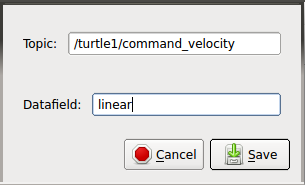
\includegraphics[scale=0.8]{img/topic_setup.png}
  }  
  \caption{Screenshot of the topic setup dialog. [re-do screenshot with rosdashboard in background]}
  \label{topic setup screenshot}
\end{figure}

ROS topics were originally not designed and developed as something the user or developer chooses graphically: They are usually created, configured and used in the source code. ROSDashboard exposes the topic setup in a graphical user interface every time a new widget is added to the dashboard. To make this as easy as possible and without much overhead, a technical solution was chosen to reduce the number of fields to be set during the topic subscription setup. Normally you have to select a topic name and a message data type. The data type can be one of the standard message types like Float, Integer, String and Boolean or a more complex message type which contains more information in a structured message. To access one data element of a message the ``datafield'' field was introduced in the graphical interface. Fig.~\ref{topic setup screenshot} shows an exemplary topic setup configuration to access the linear velocity of the \emph{/turtlesim/Velocity} message published to the topic \emph{/turtle1/command\_velocity}. Using Python's duck typing and the \emph{rostopic} module it was possible to avoid the complexity of dynamically binding message type classes during runtime and detect the message type automatically. If a topic is not yet published and thus the message type of this topic is not defined yet, the method call to \emph{rostopic} will block until the message type becomes available. To avoid blocking of the user interface a listener thread was implemented to wait until the message type for a topic becomes available (see Fig.~\ref{topic subscription}). Avoiding to manually ask the user for a message type makes the configuration of widgets easier and faster for the user, it also keeps the implementation significantly simpler, because no dynamic binding of message type classes during runtime is needed.

\begin{figure}[thpb]
  \centering
  \framebox{
    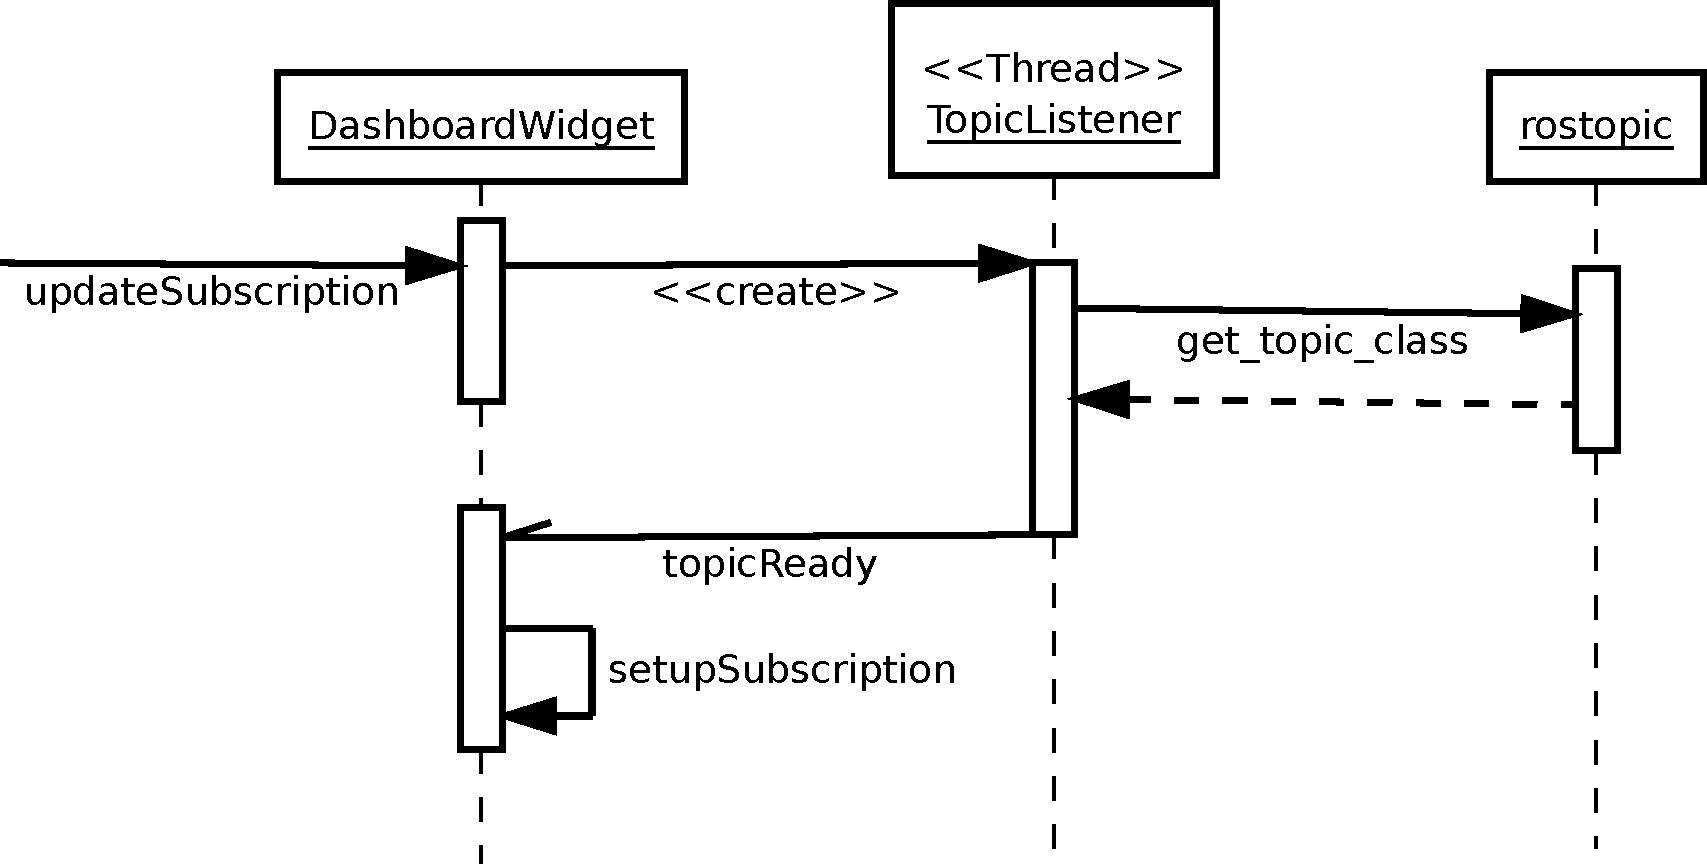
\includegraphics[scale=0.4]{diagrams/topic_subscription.pdf}
  }  
  \caption{Exemplary flow of events for asynchronous topic subscription setup.}
  \label{topic subscription}
\end{figure}

\subsection{Plugin Framework?}
I would need to implement that first...
\subsection{Example Plugin?}
Which methods need to be overwritten and how are callbacks implemented.
